\documentclass[12pt]{article}

\usepackage{sbc-template}

\usepackage{graphicx,url}

\usepackage[brazil]{babel}   
%\usepackage[latin1]{inputenc}  
\usepackage[utf8]{inputenc}  
% UTF-8 encoding is recommended by ShareLaTex

% \usepackage{natbib}
% 
% \setcitestyle{authoryear, open={((},close={))}}
     
\sloppy

\title{Sistemas Gerenciadores de Conteúdo e de Aprendizagem}

\author{Inalberth P. Santos\inst{1}, Rafael C. Gusmão\inst{1}, Ramon V. S. Bezerra\inst{1}}

\address{Instituto Federal de Educação, Ciência e Tecnologia do Maranhão\\
  Caixa Postal 15.064 -- 91.501-970 -- Porto Alegre -- RS -- Brazil
  \email{\{inalberth07, ramoncgusmao, ramonbezerra90\}@gmail.com}
}

\begin{document} 

\maketitle

\begin{abstract}
  This meta-paper describes the style to be used in articles and short papers
  for SBC conferences. For papers in English, you should add just an abstract
  while for the papers in Portuguese, we also ask for an abstract in
  Portuguese (``resumo''). In both cases, abstracts should not have more than
  10 lines and must be in the first page of the paper.
\end{abstract}
     
\begin{resumo} 
  Este meta-artigo descreve o estilo a ser usado na confecção de artigos e
  resumos de artigos para publicação nos anais das conferências organizadas
  pela SBC. É solicitada a escrita de resumo e abstract apenas para os artigos
  escritos em português. Artigos em inglês deverão apresentar apenas abstract.
  Nos dois casos, o autor deve tomar cuidado para que o resumo (e o abstract)
  não ultrapassem 10 linhas cada, sendo que ambos devem estar na primeira
  página do artigo.
\end{resumo}

\section{LMS} \label{sec:lms}

Os LMS (do inglês, \textit{Learning Management Systems}) são aplicações de \textit{software} baseadas em tecnologias Web ou não, utilizadas para 
planejar, implementar e dar suporte ao processo de aprendizagem. A TalentLMS \-- plataforma de aprendizado virtual utilizada por diversas 
organizações em segmentos distintos \-- faz em sua página uma breve explanação das 
palavras que compõem o termo\footnote{http://www.talentlms.com/what-is-an-lms/\#what-is-an-lms}:

\begin{itemize}
 \item \textbf{Learning,} porque você utiliza-os para entregar/receber programas de treinamento e/ou cursos educacionais, 
 \item \textbf{Management,} porque ajuda você a organizar estes cursos, isto é, criar, alterar,
 \item \textbf{System, } porque é um programa de computador.
\end{itemize}

Conforme \cite{lonn2009saving}, LMS são sistemas Web que permitem aos instrutores/alunos compartilhar materiais, enviar e receber tarefas, fazer 
apontamentos de aulas e se comunicar online. 


Desta maneira, observa-se consenso na literatura quanto à definição do termo, porém, apesar de 
conhecida a expressão, a mesma é empregada incorretamente com certa frequência, assim como confundida com outros dois tipos de gerenciadores: 
CMS e LCMS, os quais serão abordados nas seções seguintes.

\subsection{Origens}

Segundo \cite{watson2007learning}, a sigla LMS tem sua origem na expressão ILS (\textit{Integrated Learning System}), termo criado pela Jostens Learning, o qual faz referência a 
funcionalidades adicionais além dos recursos instrucionais, como gerenciamento de conteúdo e monitoramento. Já LMS foi utilizado pela primeira vez 
para descrever parte do sistema de gerenciamento do sistema de aprendizagem PLATO K-12.

\subsection{Características}

Em termos educacionais, constitui um LMS, conforme visto em \cite{bailey1992wanted}:

\begin{itemize}
 \item Objetos de Aprendizagem são organizados em liçõs individuais
 \item Aulas são agrupadas em um plano de ensino
 \item Um sistema de gerenciamento coleta os resultados do desempenho do estudante
 \item Aulas são disponbilizados aos alunos de acordo com o seu progresso na aprendizagem
\end{itemize}

\section{Figures and Captions}\label{sec:figs}


Figure and table captions should be centered if less than one line
(Figure~\ref{fig:exampleFig1}), otherwise justified and indented by 0.8cm on
both margins, as shown in Figure~\ref{fig:exampleFig2}. The caption font must
be Helvetica, 10 point, boldface, with 6 points of space before and after each
caption.

\begin{figure}[ht]
\centering
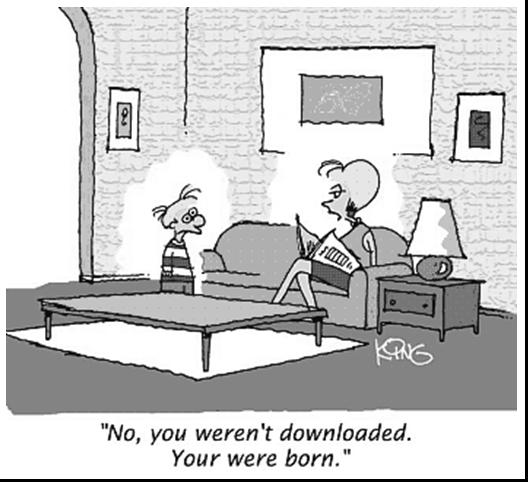
\includegraphics[width=.5\textwidth]{fig1.jpg}
\caption{A typical figure}
\label{fig:exampleFig1}
\end{figure}

\begin{figure}[ht]
\centering
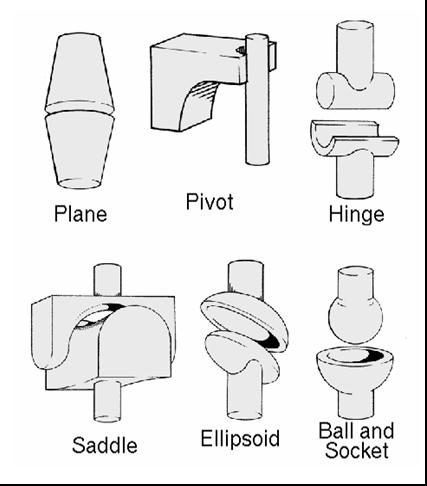
\includegraphics[width=.3\textwidth]{fig2.jpg}
\caption{This figure is an example of a figure caption taking more than one
  line and justified considering margins mentioned in Section~\ref{sec:figs}.}
\label{fig:exampleFig2}
\end{figure}

In tables, try to avoid the use of colored or shaded backgrounds, and avoid
thick, doubled, or unnecessary framing lines. When reporting empirical data,
do not use more decimal digits than warranted by their precision and
reproducibility. Table caption must be placed before the table (see Table 1)
and the font used must also be Helvetica, 10 point, boldface, with 6 points of
space before and after each caption.

\begin{table}[ht]
\centering
\caption{Variables to be considered on the evaluation of interaction
  techniques}
\label{tab:exTable1}
\smallskip
\begin{tabular}{|l|c|c|}
\hline
& Value 1 & Value 2\\[0.5ex]
\hline
&&\\[-2ex]
Case 1 & 1.0 $\pm$ 0.1 & 1.75$\times$10$^{-5}$ $\pm$ 5$\times$10$^{-7}$\\[0.5ex]
\hline
&&\\[-2ex]
Case 2 & 0.003(1) & 100.0\\[0.5ex]
\hline
\end{tabular}
\end{table}

\section{Images}

All images and illustrations should be in black-and-white, or gray tones,
excepting for the papers that will be electronically available (on CD-ROMs,
internet, etc.). The image resolution on paper should be about 600 dpi for
black-and-white images, and 150-300 dpi for grayscale images.  Do not include
images with excessive resolution, as they may take hours to print, without any
visible difference in the result. 

\section{References}

Bibliographic references must be unambiguous and uniform.  We recommend giving
the author names references in brackets, e.g. \cite{knuth:84},
\cite{boulic:91}, and \cite{smith:99}.

The references must be listed using 12 point font size, with 6 points of space
before each reference. The first line of each reference should not be
indented, while the subsequent should be indented by 0.5 cm.

\bibliographystyle{sbc}
\bibliography{referencias}

\end{document}
